The purpose of this analysis is to verify that \texttt{\getsoftwarename{}} is able
to reproduce the correct pseudo-acceleration response spectrum when
using synthetic acceleration time histories generated using the
stochastic ground motion model option as the seismic event. The maximum
pseudo-acceleration for a single-degree-of-freedom system with varying
natural frequencies calculated by \texttt{\getsoftwarename{}} is compared to the
values predicted by \texttt{smelt} as well as the geometric mean
of the four NGA-West2 ground motion prediction equations (GPMEs)
that account for soil sites. The scenario considered in this verification
example is an event with a Moment Magnitude ($M_W$) of 6.5, closest-to-site
rupture distance ($R_{\textrm{rupt}}$) of 20 km, and average shear-wave velocity in the top
30 m of soil ($V_{s30}$) equal to 400 m/s.\\

The single-degree-of-freedom system was input using the MDOF option as
the Building Model Input in \texttt{\getsoftwarename{}}. Here, the mass was set to
unity and the damping ratio to 5\%. The story stiffness was modified
to set the natural frequency of the system in order to calculate the
response spectrum. The structural response was calculated for 10
sample synthetic acceleration time histories for each structural
period and compared to those from \texttt{smelt} and the GMPEs, as
shown in \Cref{fig:stochastic_validation}. As can be seen in this
figure, the spectral response calculated by \texttt{\getsoftwarename{}} falls
within the mean plus/minus one sigma bounds of the GMPEs and
\texttt{smelt} while tending toward the mean. This produces the
expected result as \texttt{\getsoftwarename{}} is calling \texttt{smelt} in the
backend to generate the synthetic motions. The full validation of
\texttt{smelt} in implementing the predictive stochastic model
proposed by Vlachos et al. (2018) \cite{vlachos2018predictive} can be
found in the
\href{https://github.com/NHERI-SimCenter/smelt}{library
  documentation}.

\begin{figure}[!htbp]
  \centering {
    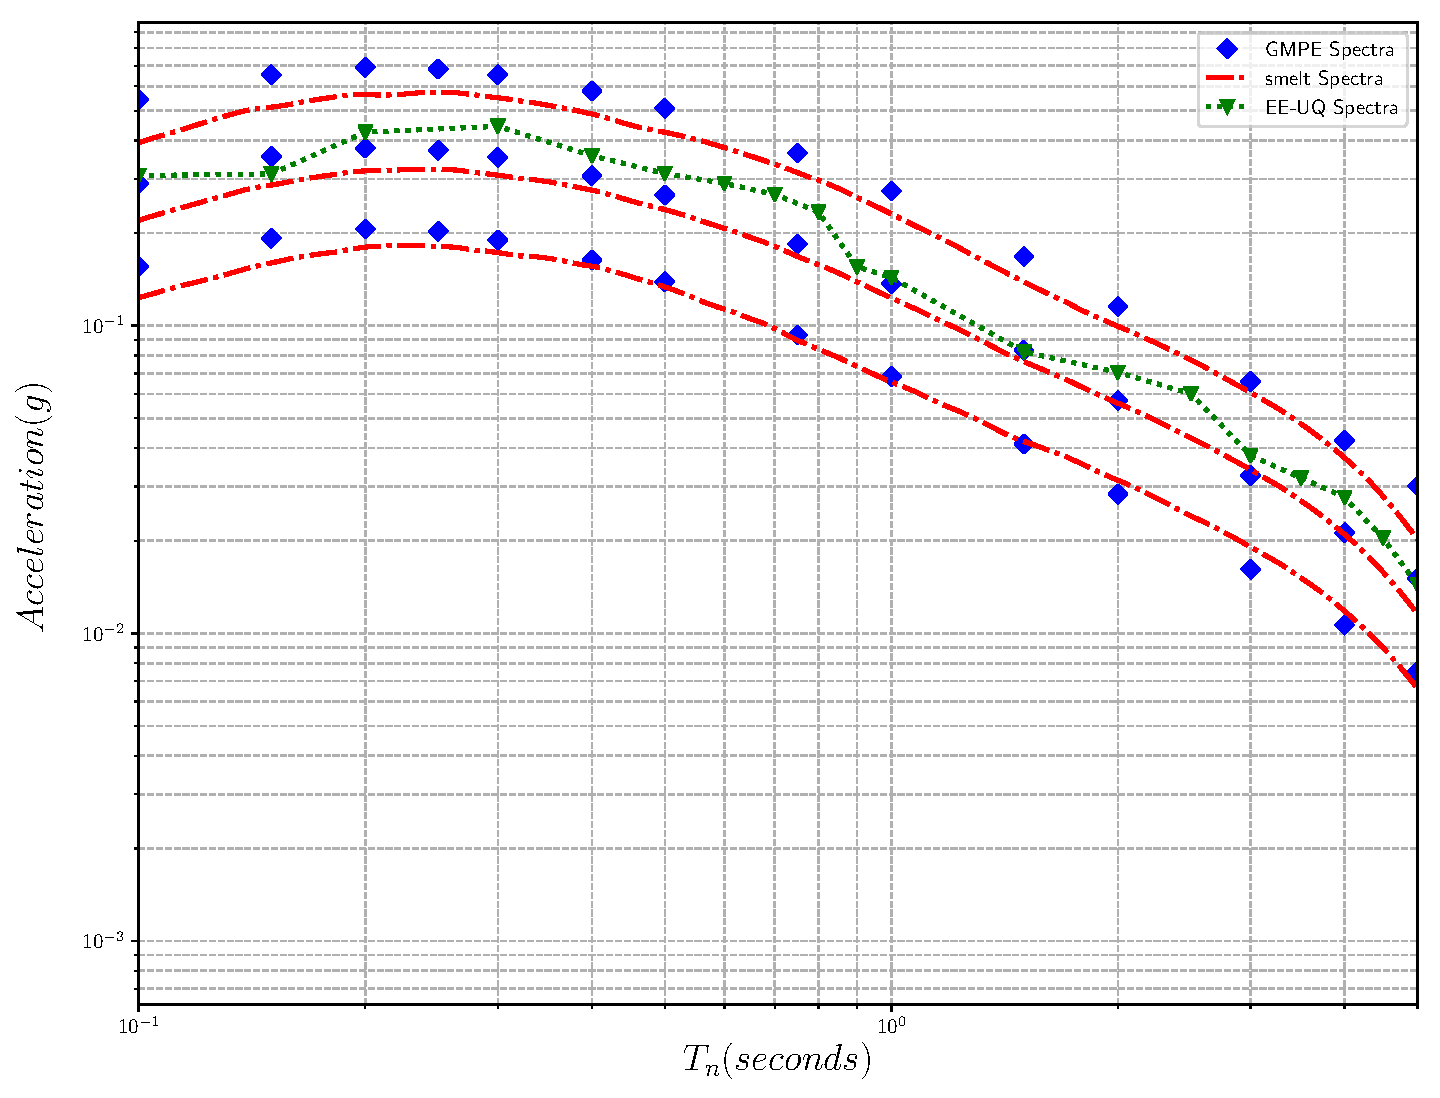
\includegraphics[width=0.8\textwidth]
    {ver_and_val/figures/M65R20V400.pdf} }
  \caption[Response Spectra generated using NGA-West2
    GMPEs, \texttt{smelt} \& \texttt{\getsoftwarename{}} for $M_W = 6.5$, $R_{\textrm{rupt}}
    = 20\;\textrm{km}$, and $V_{s30} = 400\;\textrm{m/s}$]
    {Response Spectra generated using NGA-West2
    GMPEs, \texttt{smelt} \& \texttt{\getsoftwarename{}} for $M_W = 6.5$,
    closest-to-site distance $R_{\textrm{rupt}} = 20\;\textrm{km}$, and average shear-wave
    velocity $V_{s30} = 400\;\textrm{m/s}$. The \texttt{smelt} and GMPE
    spectra show the mean and mean plus/minus one logarithmic standard
    deviation. The GMPE spectra are based on the geometric mean of the
    four NGA-West2 models that account for site soil
    conditions. The \texttt{smelt} spectra are based on an ensemble of
    1000 synthetic ground motions. \texttt{\getsoftwarename{}} response values are
    based on the mean pseudo-acceleration for 10 synthetic ground
    motion samples per period, $T_n$}
  \label{fig:stochastic_validation}
\end{figure}
